Ogni applicazione web è composta da due parti che collaborano per riuscire a offrire all'utente quello che ha richiesto: \emph{backend} e \emph{frontend}. Questa sezione parlerà di come è stato studiato e, successivamente, implementato il frontend.

\subsection{Studio iniziale}
	Clusterify nasce per essere un'applicazione \emph{user-centered}: si sono delineate tre \emph{personas} in grado di rappresentare i differenti utilizzi che questa potesse supportare:
	\begin{itemize}
		\item Gigi Parigi \emph{(studente di informatica - maschio - 20 anni)}: Gigi si è appena diplomato al liceo scientifico della sua città e si è immatricolato per seguire il corso in scienze informatiche. Utilizza Twitter sopratutto per rimare aggiornato sulle ultime notizie circa il mondo dell'open source. Si rende conto di leggere tweet di poco interesse quando gli utenti che segue parlano della propria vita privata.
		\item Rossella Secchi \emph{(giornalista - femmina - 25 anni)}: Rossella è giornalista presso un emergente giornale online ed utilizza spesso Twitter per seguire il susseguirsi degli avvenimenti prima che questi vengano pubblicati da altri giornali. Il suo scopo è quello di riuscire a lanciare le notizie prima degli altri. Ritiene che avere le notizie raggruppate per argomento le salverebbe molto tempo speso in ricerca.
		\item Giovanni Fantuzzo \emph{(fanatico di serie TV - maschio - 23 anni)}: Giovanni dopo aver smesso di guardare i cartoni animati ha capito che le serie TV sarebbero state un valido sostituto. Utilizza Twitter per seguire le news legate al campo: le interviste che fanno agli attori, nuovi rumors  riguardanti nuove serie proposte e via dicendo. Sarebbe felice di poter avere tutte queste serie TV divise l'una dall'altra.
	\end{itemize}

	Tutte queste personas sono legate al mondo di Twitter: utilizzano questo social network ma in modi diversi. Si può dedurre che questa piattaforma deve essere facile da utilizzare e, soprattutto, accessibile anche ad utenti non molto legati al campo dell'informatica. È emerso il bisogno di mostrare una netta divisione tra i vari topic, rendendo le partizioni riconoscibili a colpo d'occhio. Infine, i gruppi devono permettere di essere esplorati portandoti ai tweet che lo hanno formato.

	Sono stati abbozzati dei \emph{mockup} pensando come queste personas si sarebbero comportate all'interno della piattaforma.

	L'idea era quella di creare un \emph{wizard} che permettesse in pochi \emph{click} di ottenere il risultato finale:

        	\begin{figure}[p]
		\textbf{Pagina di benvenuto}: pagina dove sarà possibile ottenere informazioni su Clusterify e dove sarà possibile loggarsi. Si è deciso di permettere di utilizzare l'account Twitter come unico modo per registrarsi/loggarsi con il fine di semplificare l'interfaccia.\\

        		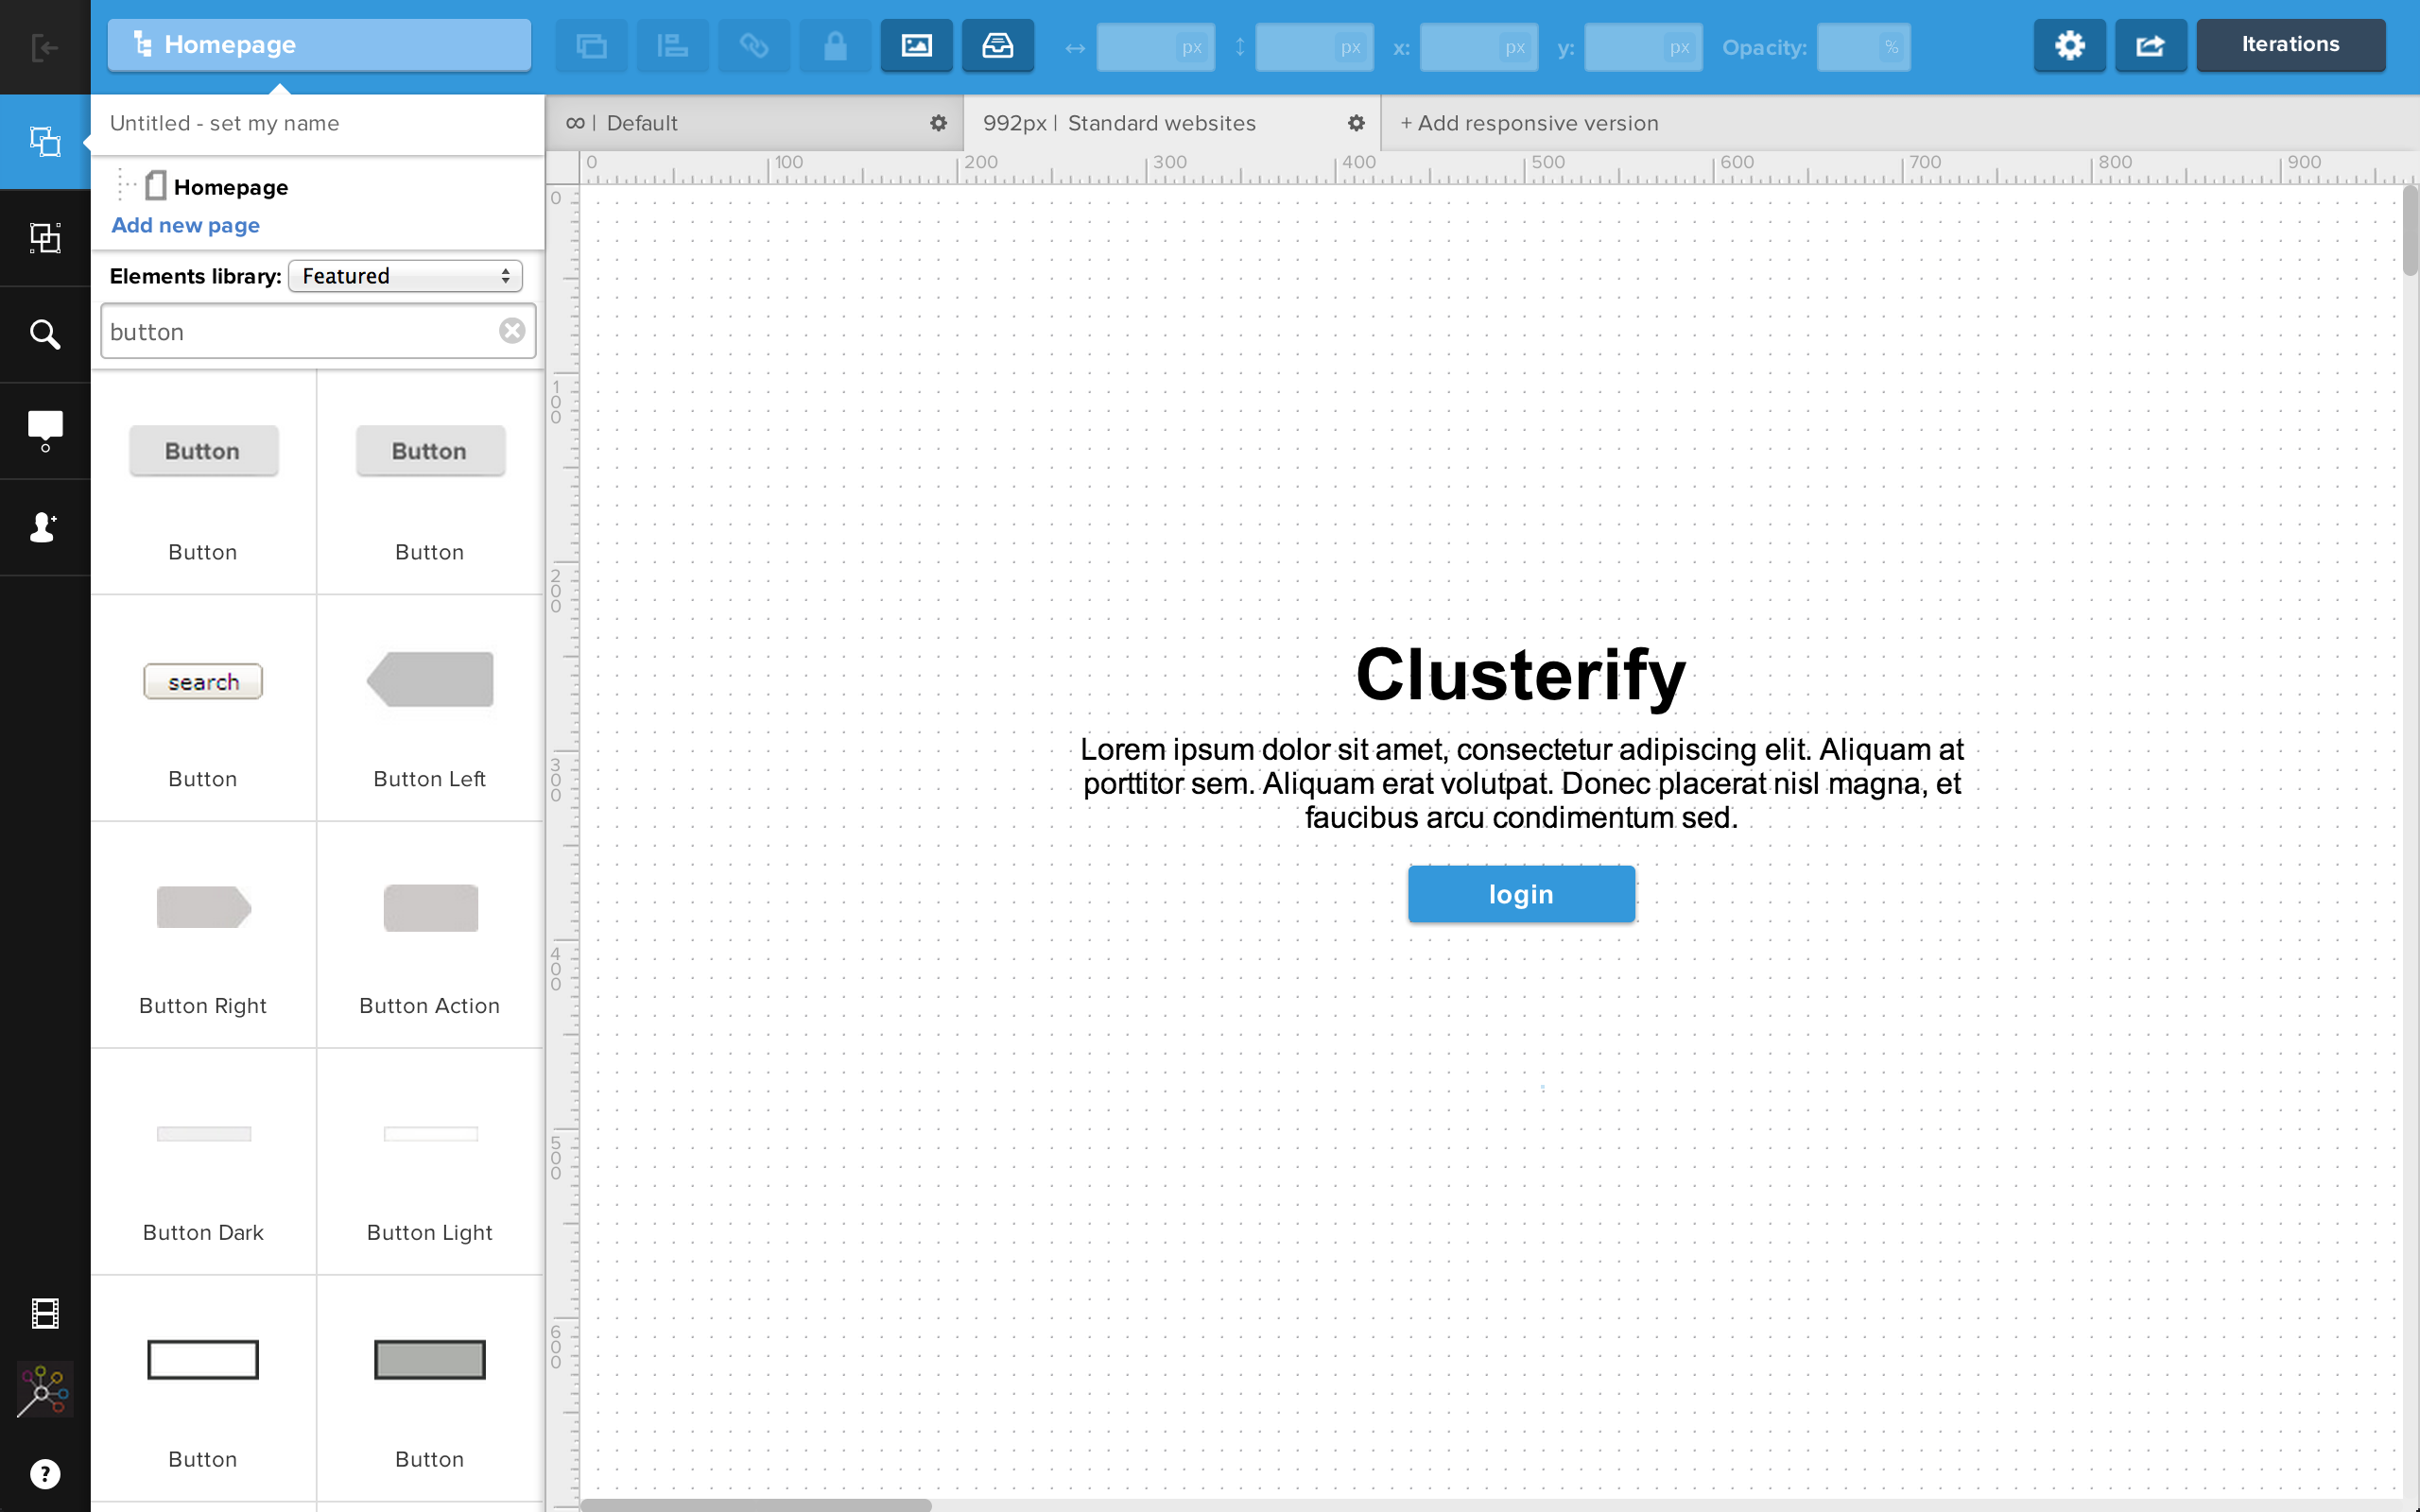
\includegraphics[width=\textwidth]{img/mockup/welcome.png}
        	\end{figure}

        	\begin{figure}[p]
		\textbf{Inserimento email}: pagina dove si richiederà di inserire la propria mail.\\

        		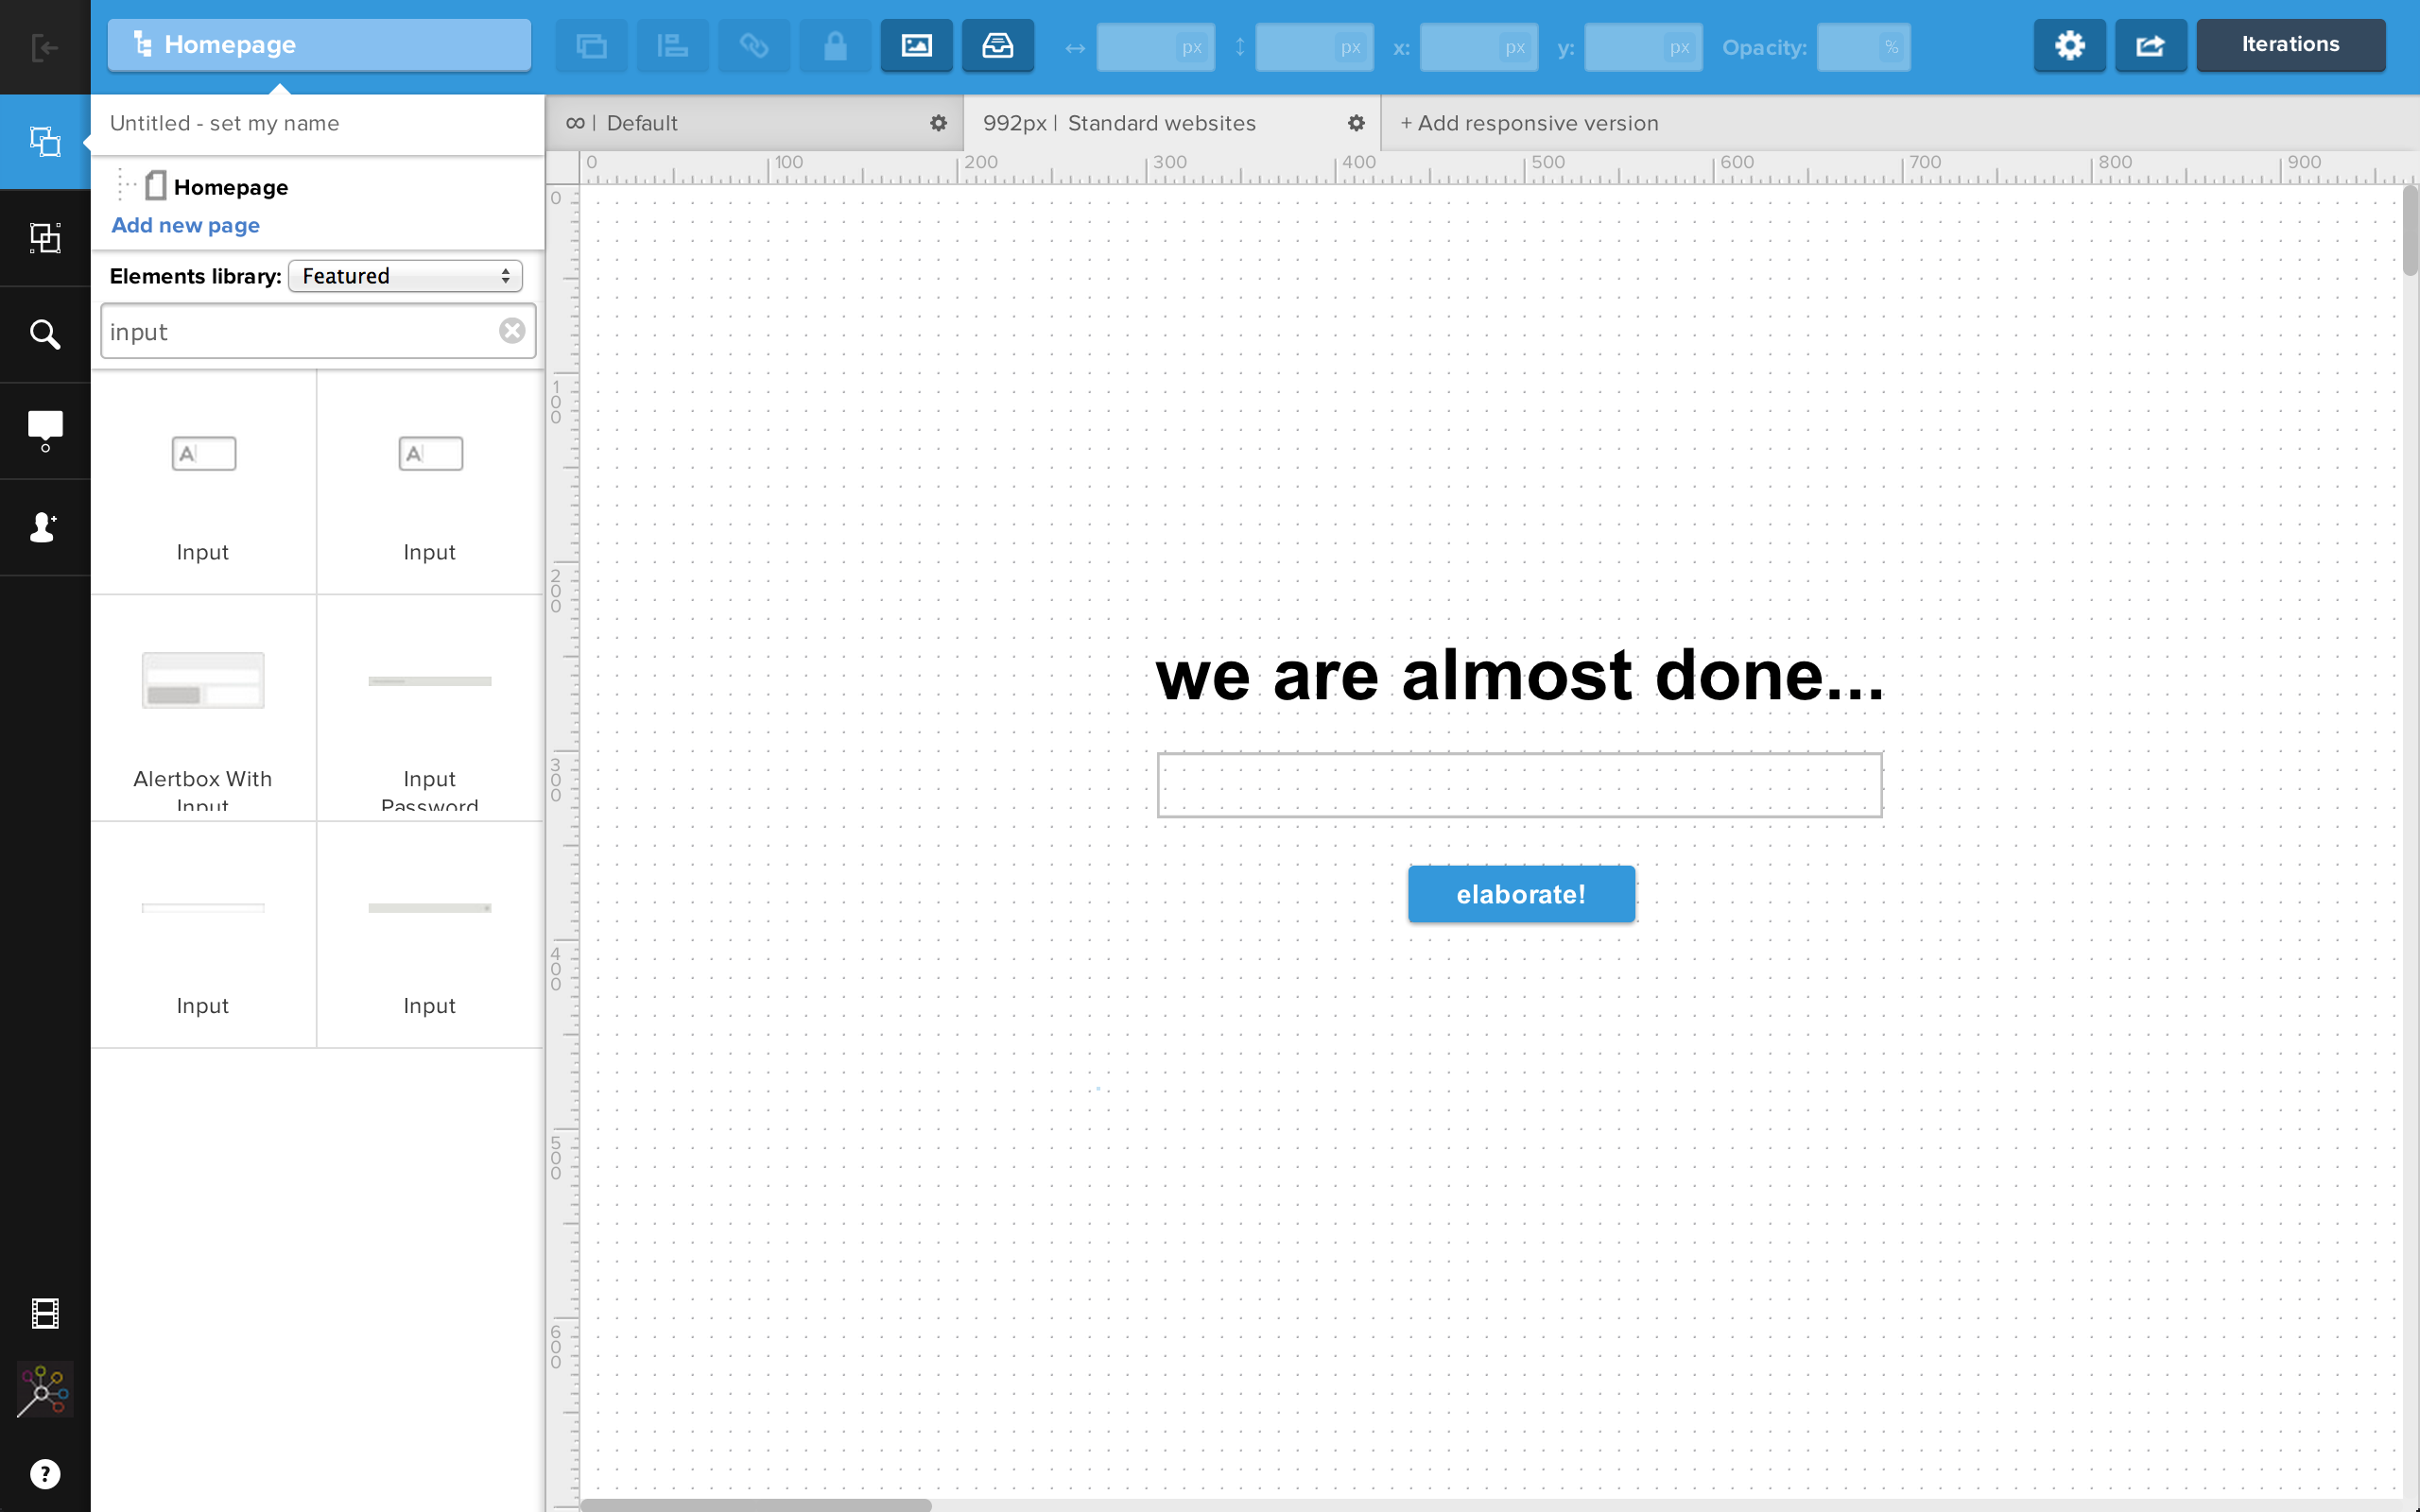
\includegraphics[width=\textwidth]{img/mockup/email.png}
        	\end{figure}

        	\begin{figure}[p]
		\textbf{Stato dell'elaborazione}: pagina che mostra all'utente lo stato dell'ultima elaborazione che questo ha lanciato.\\

        		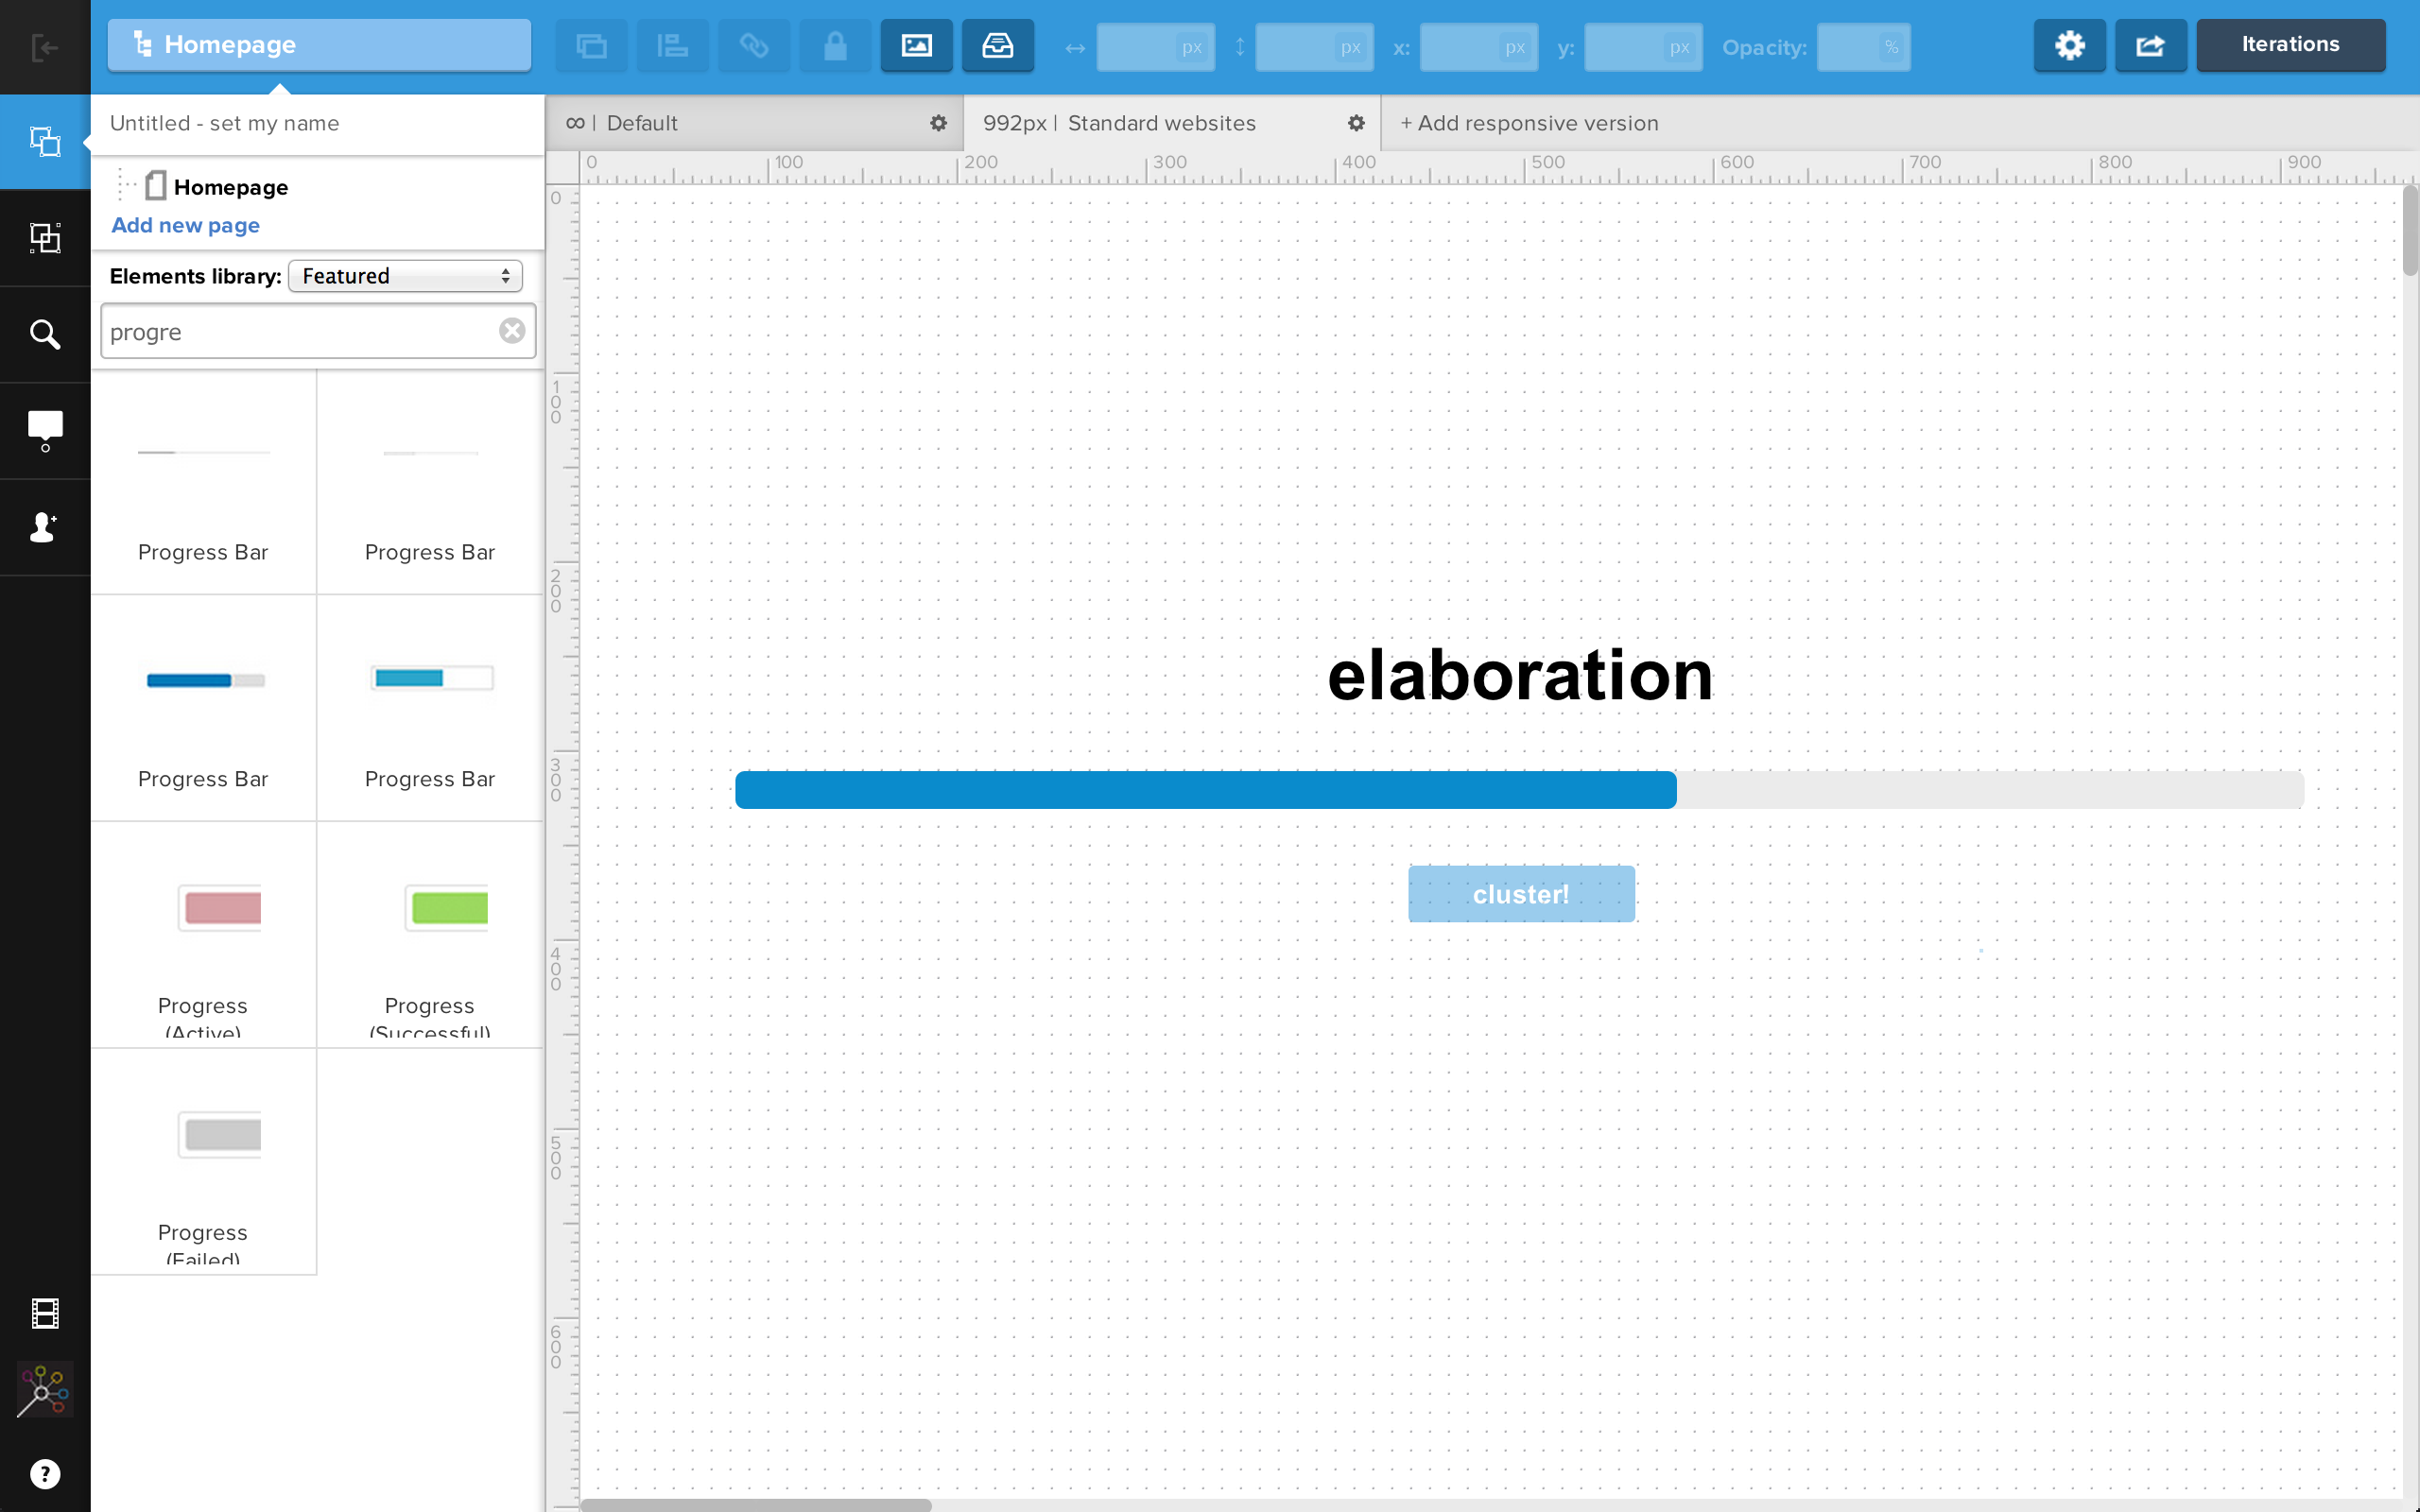
\includegraphics[width=\textwidth]{img/mockup/process.png}
        	\end{figure}

        	\begin{figure}[p]
		\textbf{Elaborazione}: pagina che mostra il risultato dell'elaborazione.\\

        		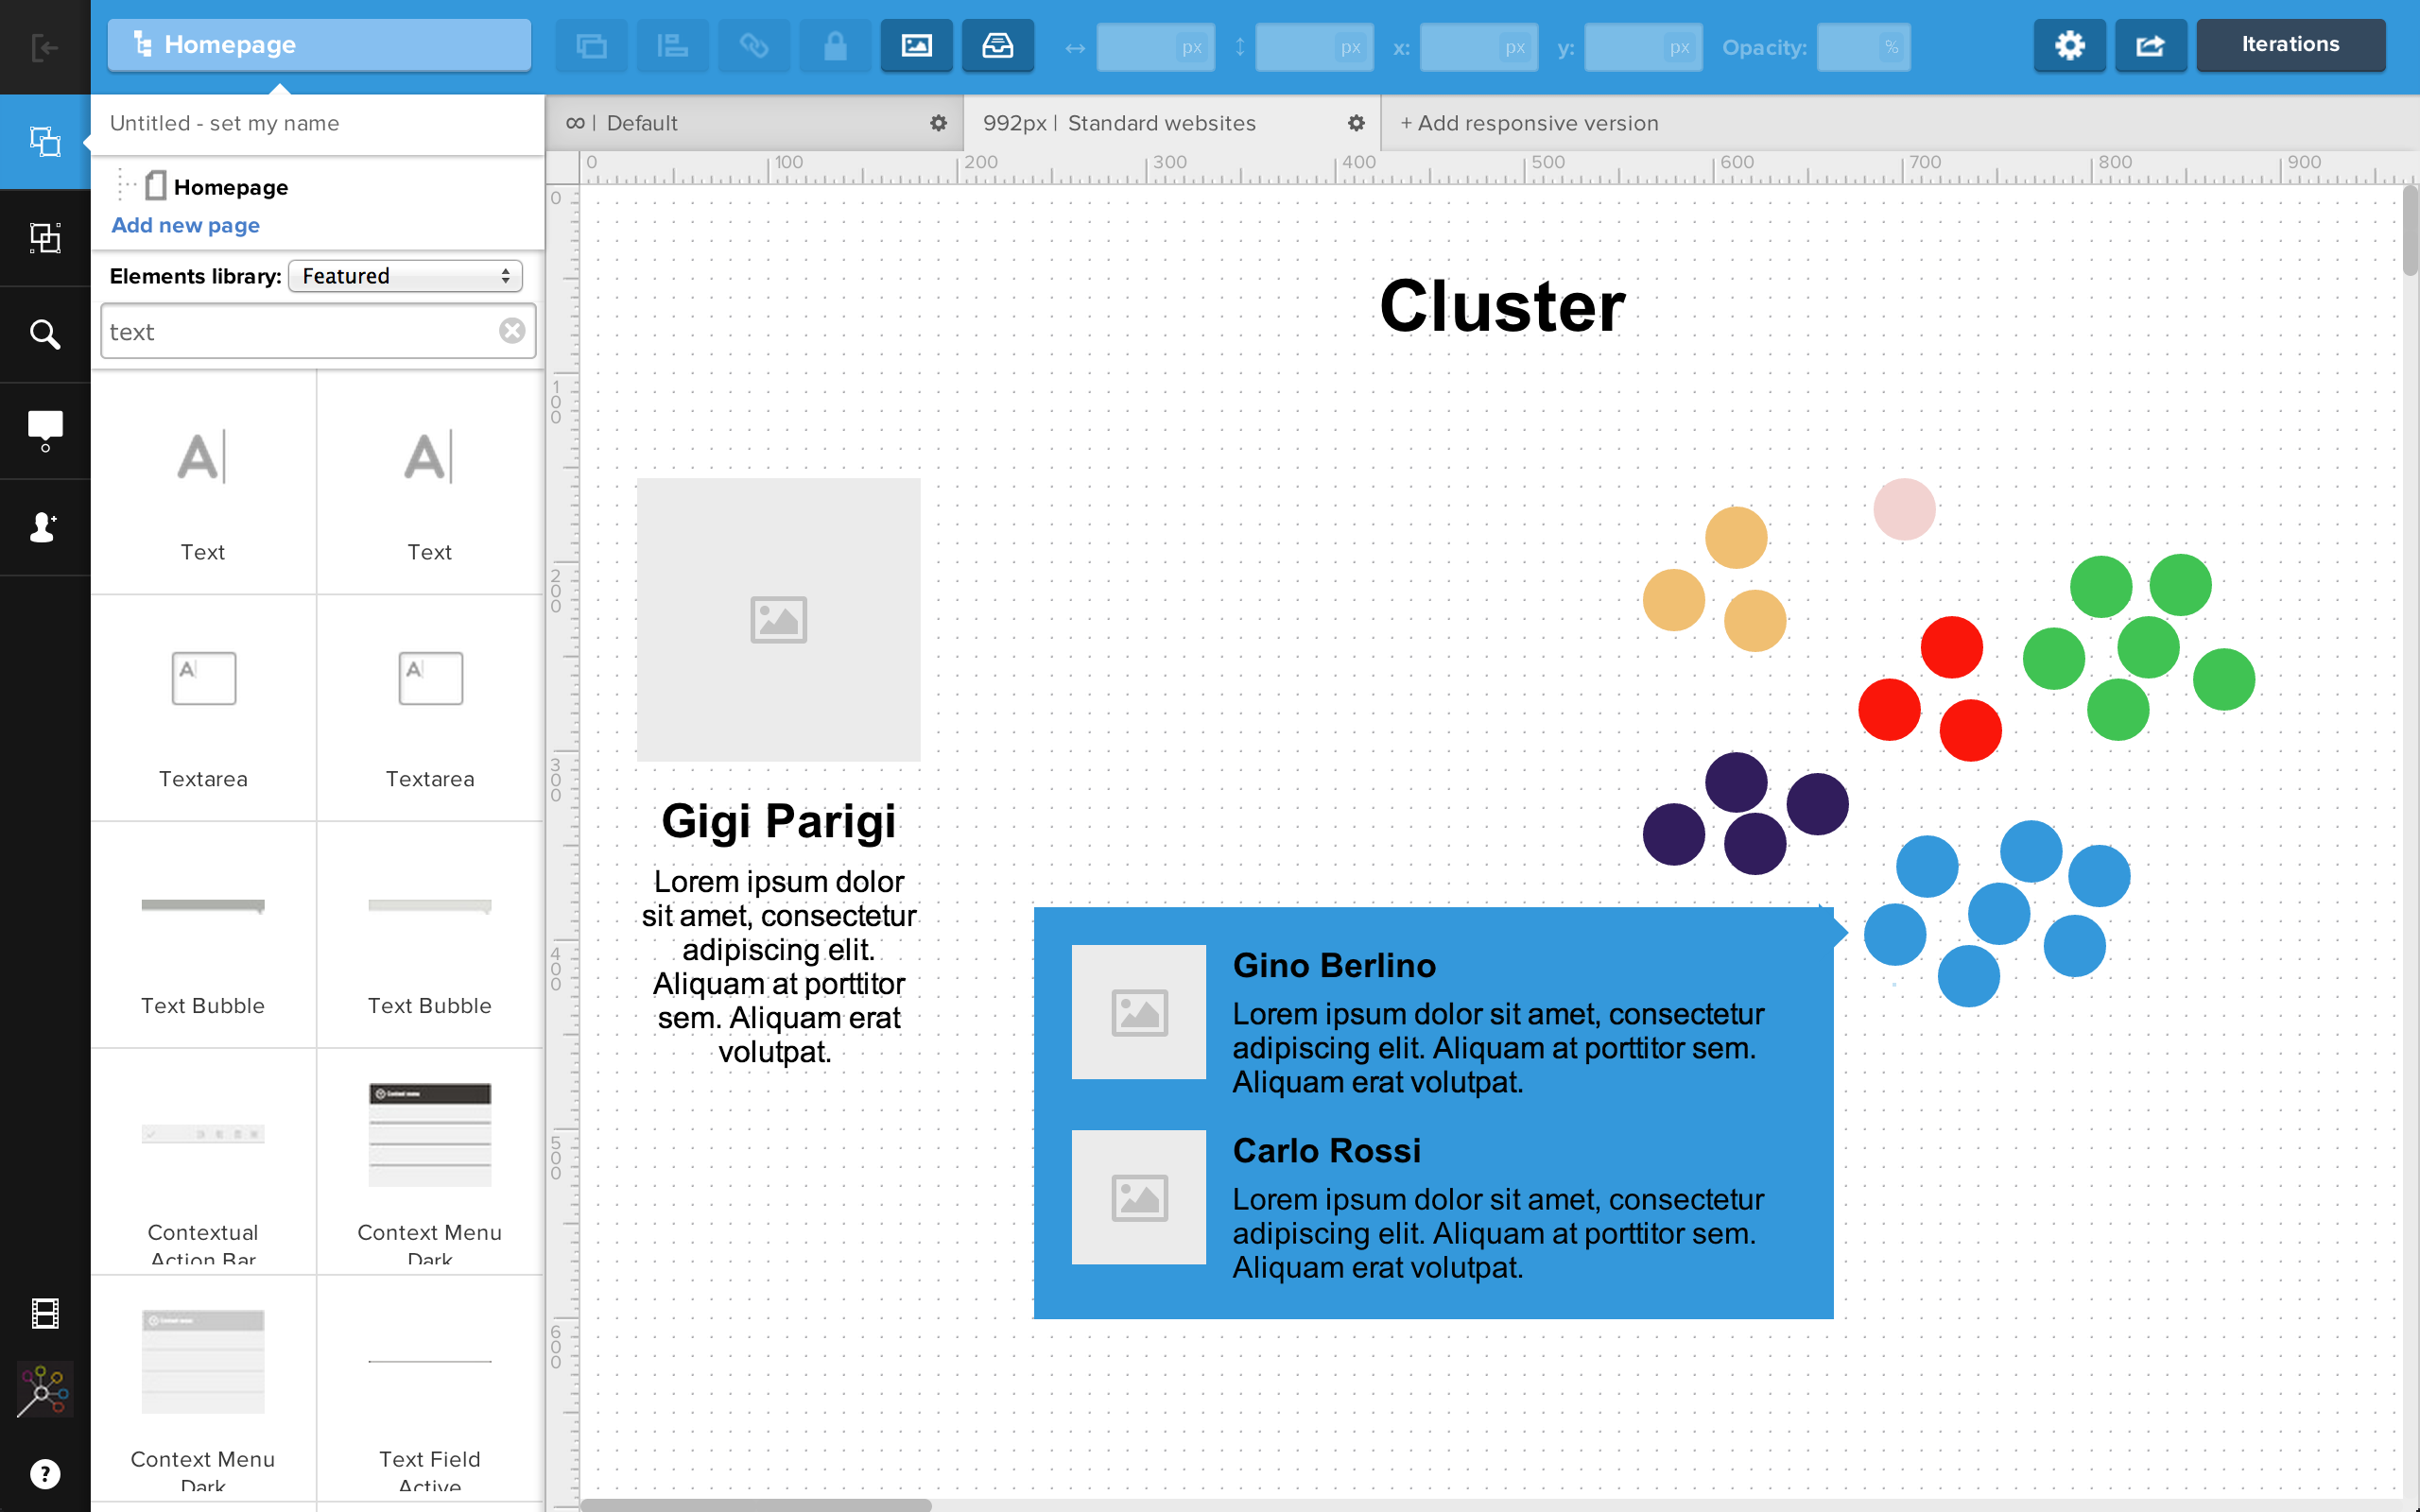
\includegraphics[width=\textwidth]{img/mockup/elaboration.png}
        	\end{figure}
            
	\newpage
         Questi mockup sono stati proposti a cinque utenti che hanno permesso di capire alcuni problemi che erano stati introdotti.
            
	\begin{itemize}
		\item  Nella pagina di richiesta dell'email non si capiva cosa venisse chiesto agli utenti. Si è decido di aggiungere degli aiuti visivi che permetteranno loro di capire.
            
            	\item Nella pagina dedicata allo stato dell'elaborazione, gli intervistati non capivano cosa Clusterify stesse facendo, nemmeno che questo processo sarebbe continuato anche se loro avessero chiuso la pagina e che un'email gli avrebbe notificati quando questo sarebbe finito. Si è deciso di aggiungere una scritta che chiarirà il comportamento di Clusterify. 
                        
            	\item Nella pagina dedicata alla visualizzazione del cluster, viene dato poco spazio ai tweet mentre questi dovrebbero essere l'elemento fondamentale della piattaforma.
            
            	\item Si è notata la necessità di avere una pagina con le elaborazioni passate.
            \end{itemize}
            

\subsection{Studio finale}        
	Clusterify utilizza come framework di base Bootstrap -- \url{http://getbootstrap.com/} --, utile per alcune componenti quali la griglia ed i menù \emph{dropdown}.
        
	Per la parte di \emph{data visualization} utilizzerà d3 -- \url{http://d3js.org/} --, una libreria scritta in JavaScript utile per maneggiare dati e permettere la loro visualizzazione.
        
	Dopo aver capito i problemi riscontrati nei mockup dai primi intervistati, si è implementato Clusterify.

        	\begin{figure}[p]
		\textbf{Pagina di benvenuto}: landing page che offre la possibilità di registrarsi o di effettuare log in. Questa è anche la pagina dove si viene ridirezionati quando si richiede una visualizzazione di una pagina bloccata.\\

        		
\includegraphics[width=\textwidth]{img/clusterify/welcome.png}
        	\end{figure}
        
        	\begin{figure}[p]
		\textbf{Inserimento email}: nel momento in cui un utente si registra, viene domandato di inserire una propria email. L'indirizzo è necessario per contattare l'utente quando un'elaborazione termina.\\

        		
\includegraphics[width=\textwidth]{img/clusterify/email.png}
        	\end{figure}
        
        	\begin{figure}[p]
		\textbf{Stato dell'elaborazione}: quando un utente lancia un'elaborazione viene mostrata questa \emph{progress-bar}. Il processo assume la struttura del backend. Il passo illuminato è quello che sta venendo elaborato in quel momento.\\

        		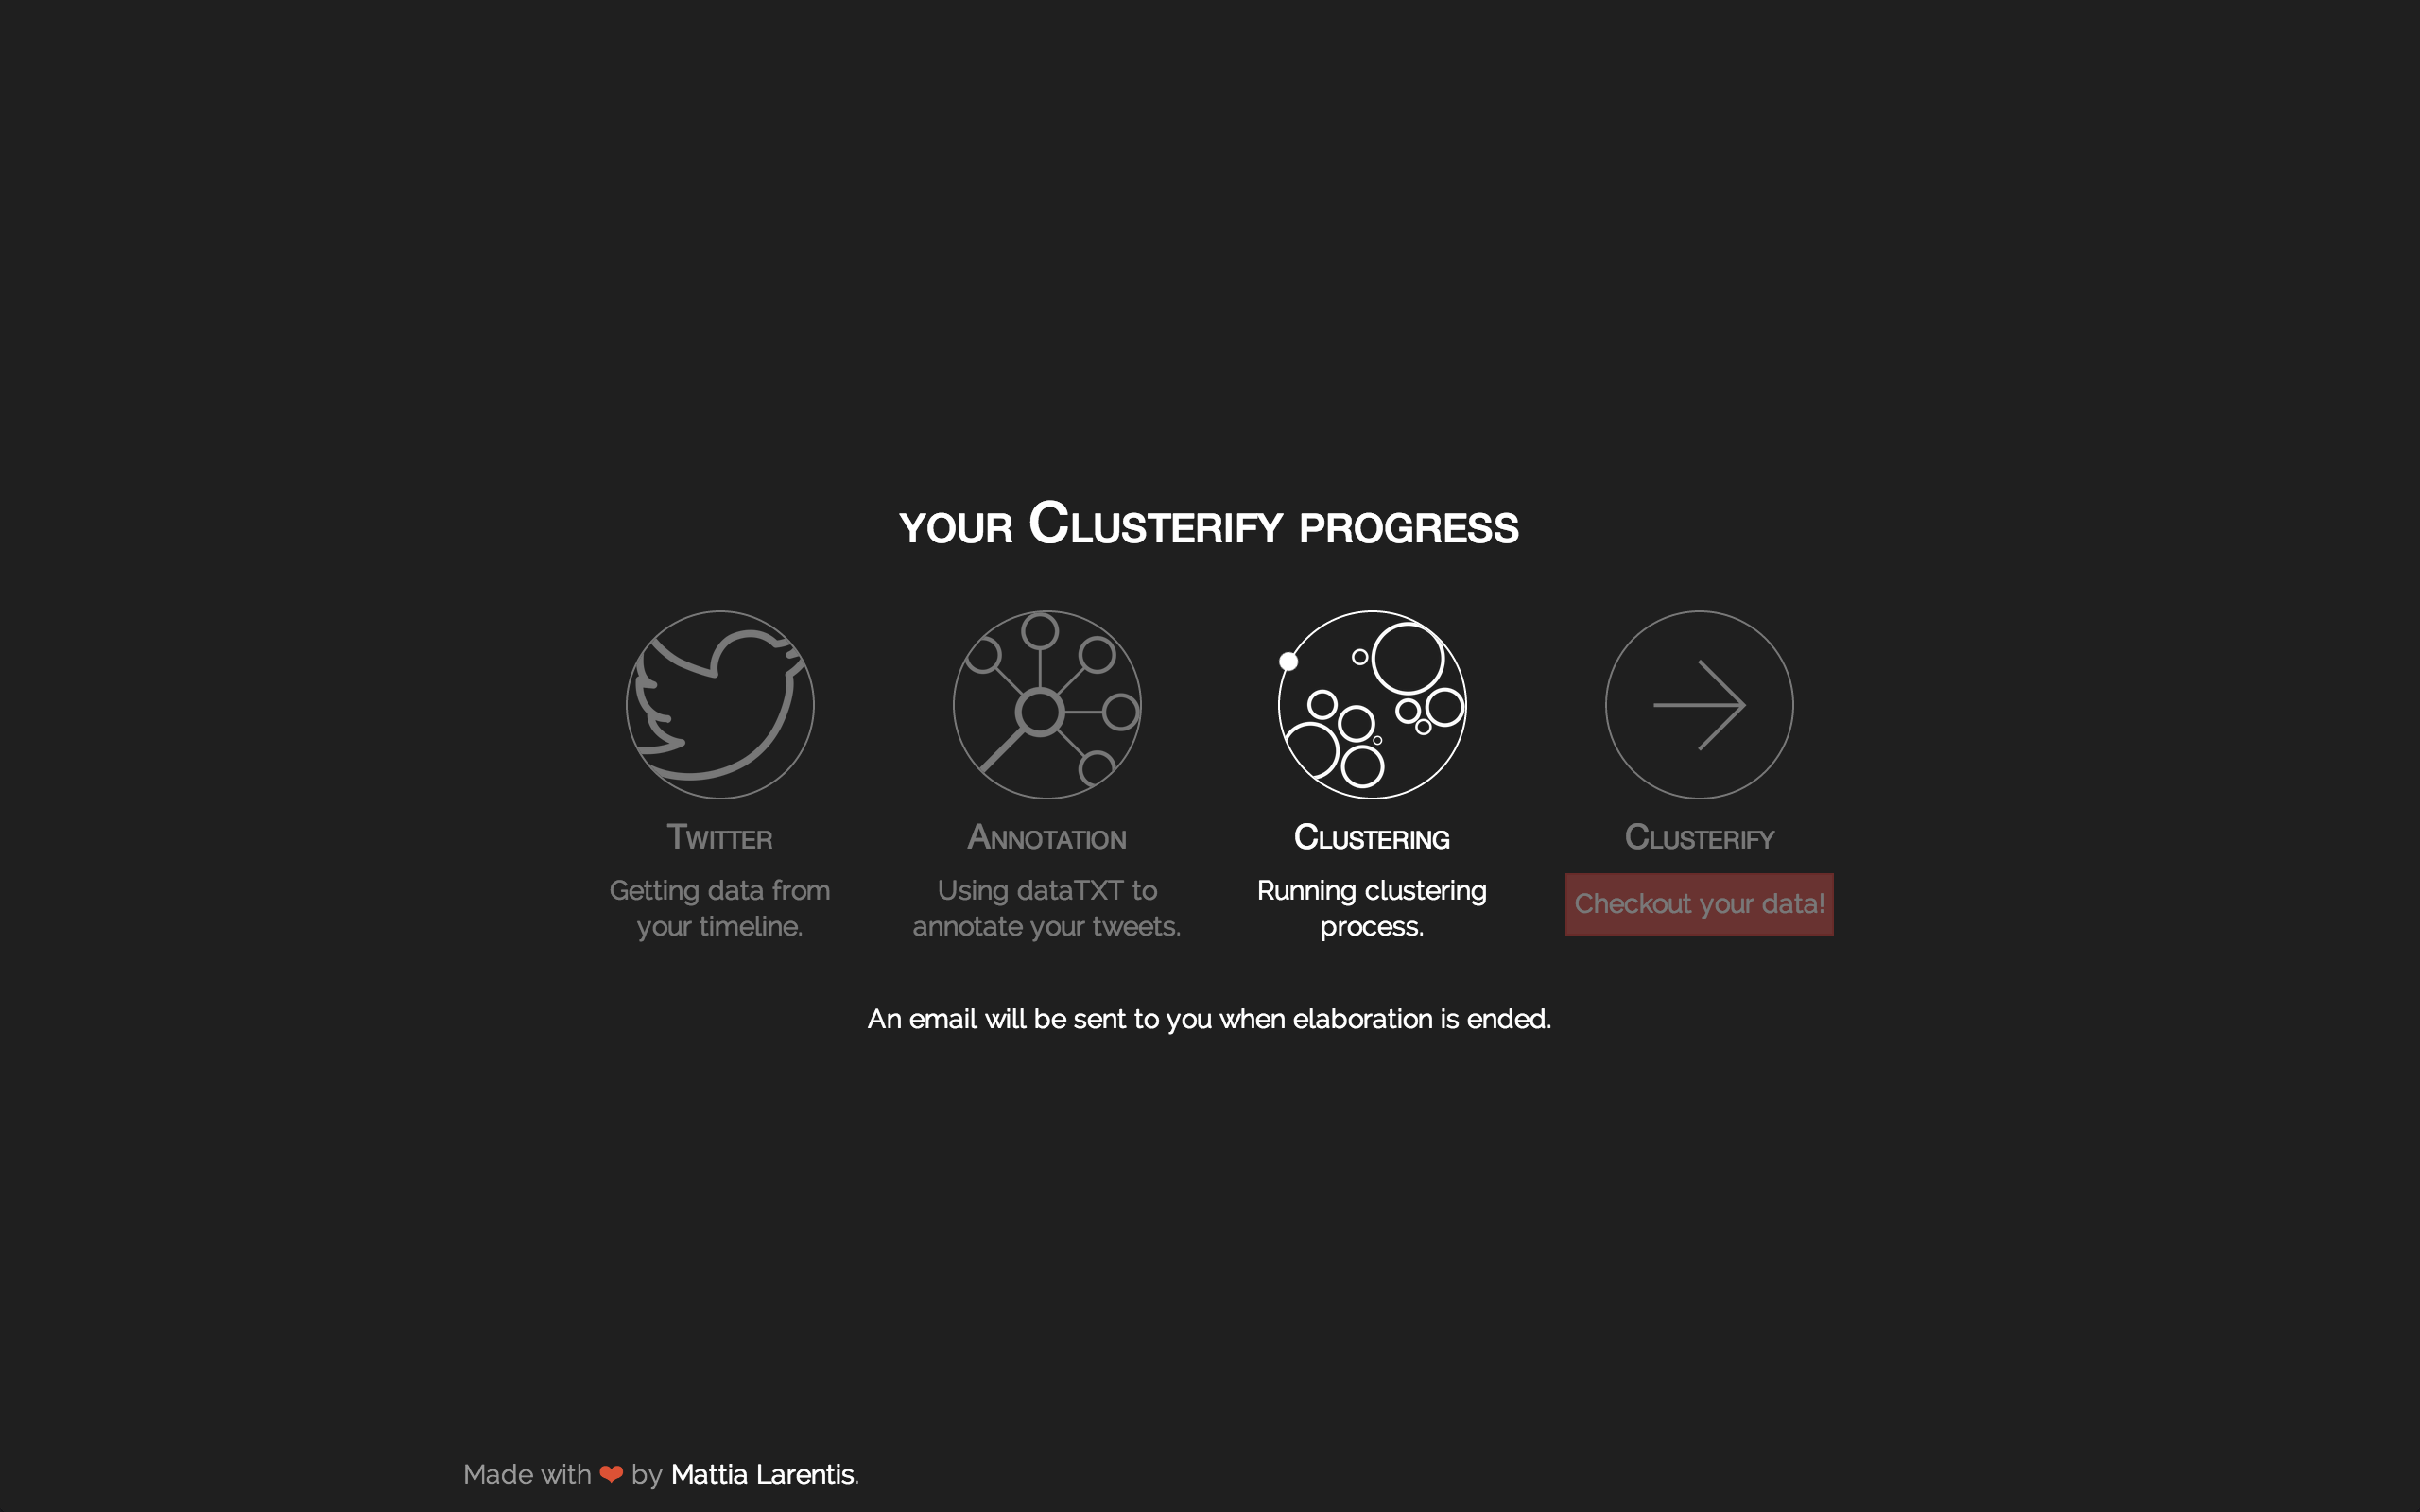
\includegraphics[width=\textwidth]{img/clusterify/process.png}
        	\end{figure}
        
        	\begin{figure}[p]
		\textbf{Elaborazione}: pagina che mostra il cluster calcolato da Clusterify. Dal menù in alto è possibile lanciare una nuova elaborazione oppure visualizzare lo storico.\\

        		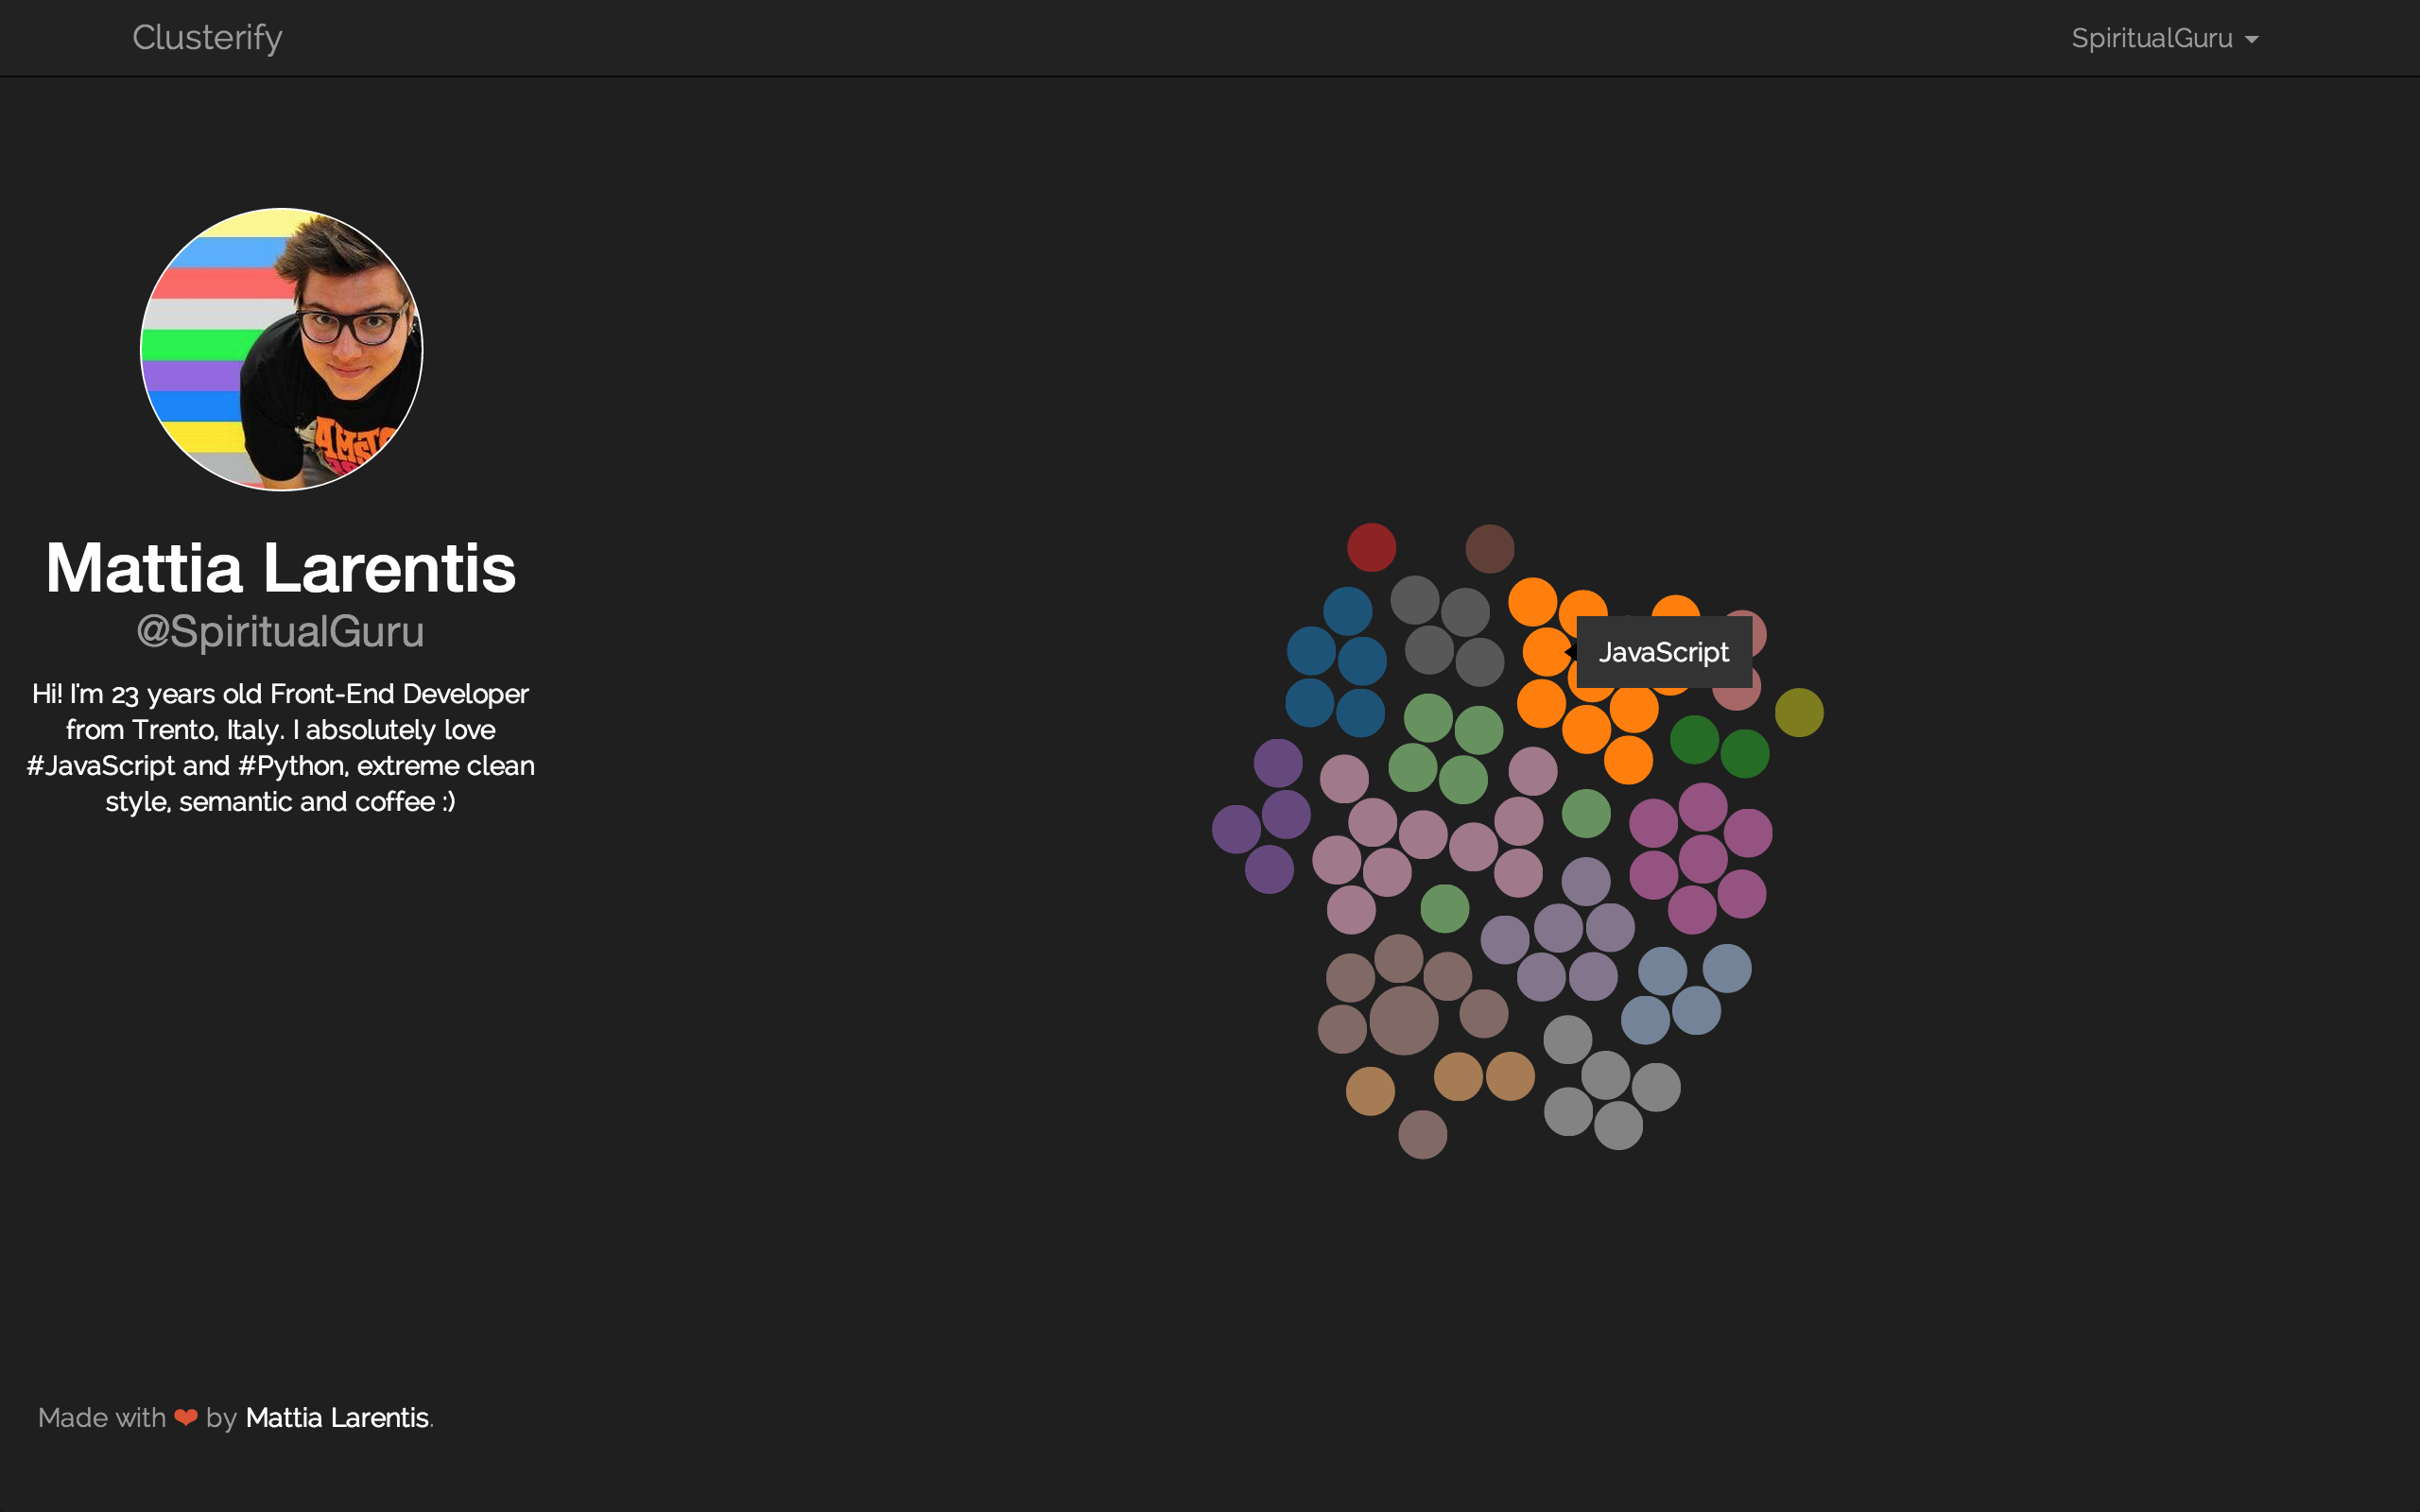
\includegraphics[width=\textwidth]{img/clusterify/elaboration.png}
        	\end{figure}
        
        	\begin{figure}[p]
		\textbf{Tweet}: da ``Elaborazione'' è possibile navigare ogni cluster clickando su un qualsiasi elemento che lo compone. Quando questo succede, una finestra modale si apre e permette di leggere tutti i tweet che sono stati raggruppati. Un tweet può appartenere a più cluster. Se un tweet viene premuto, si viene mandati alla pagina di Twitter dove il tweet risiede.\\

        		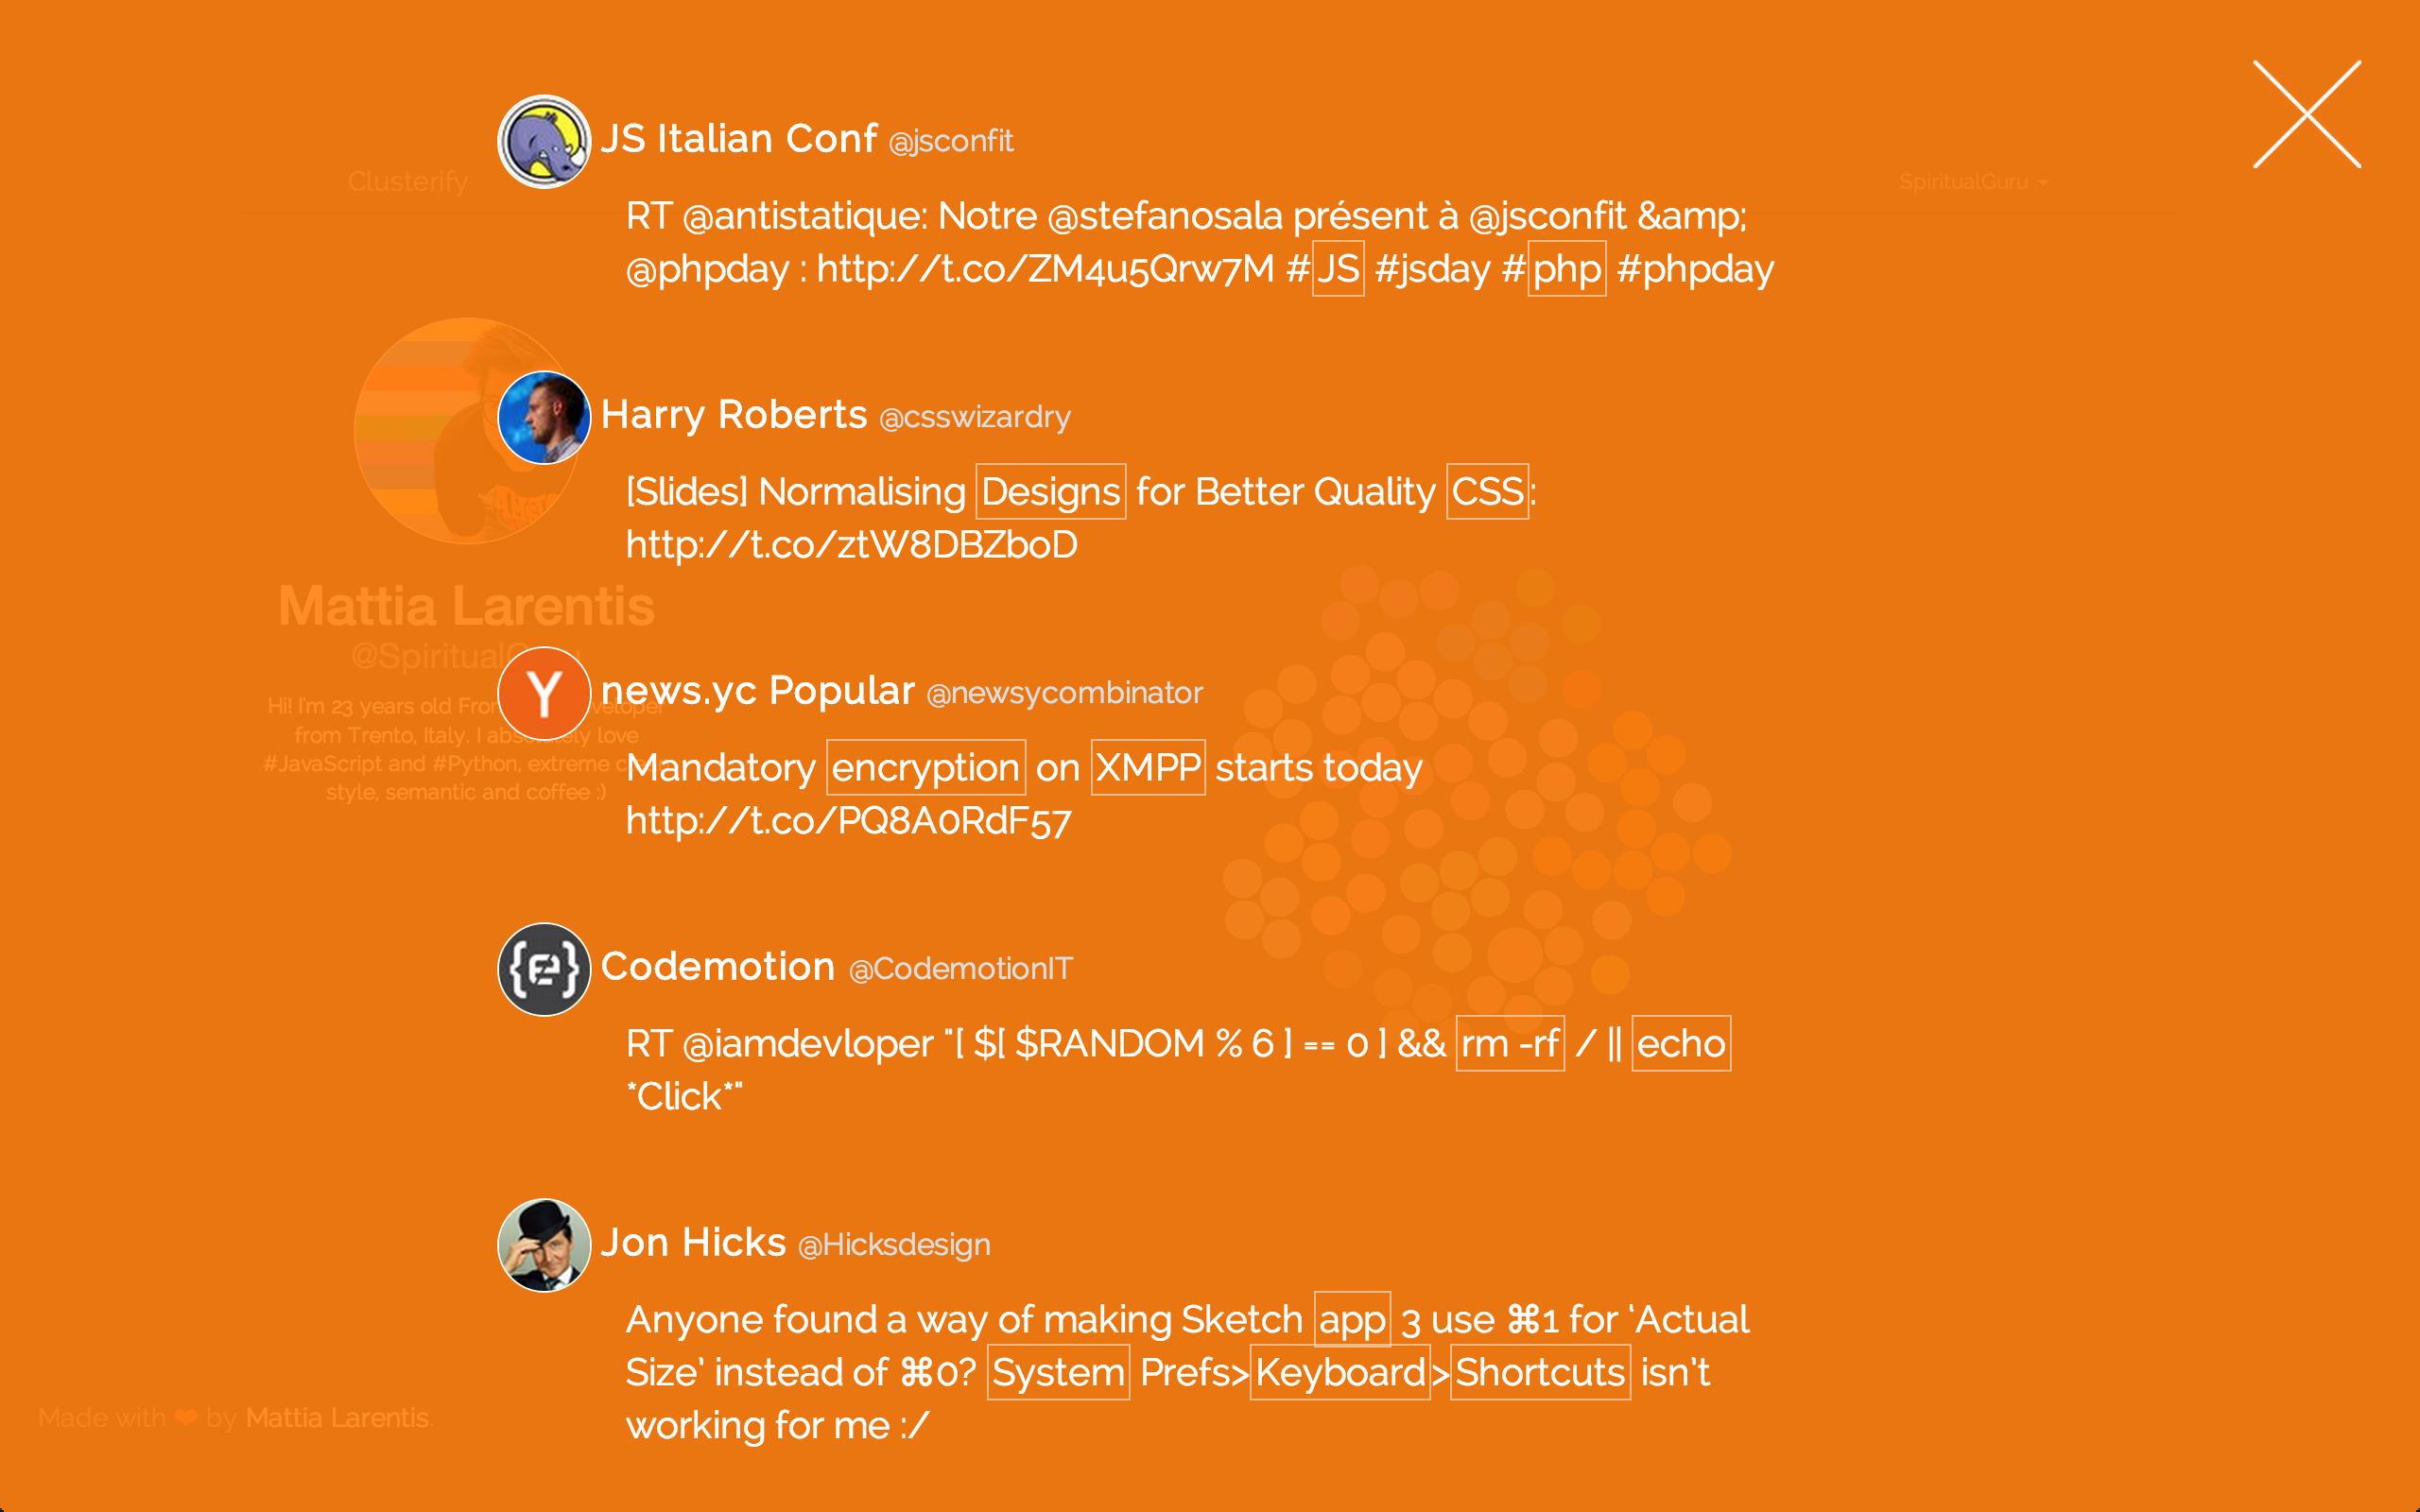
\includegraphics[width=\textwidth]{img/clusterify/tweet.png}
        	\end{figure}
        
        	\begin{figure}[p]
		\textbf{Storico delle elaborazioni}: pagina dove sono visibili tutte le elaborazioni che un utente ha lanciato.\\

        		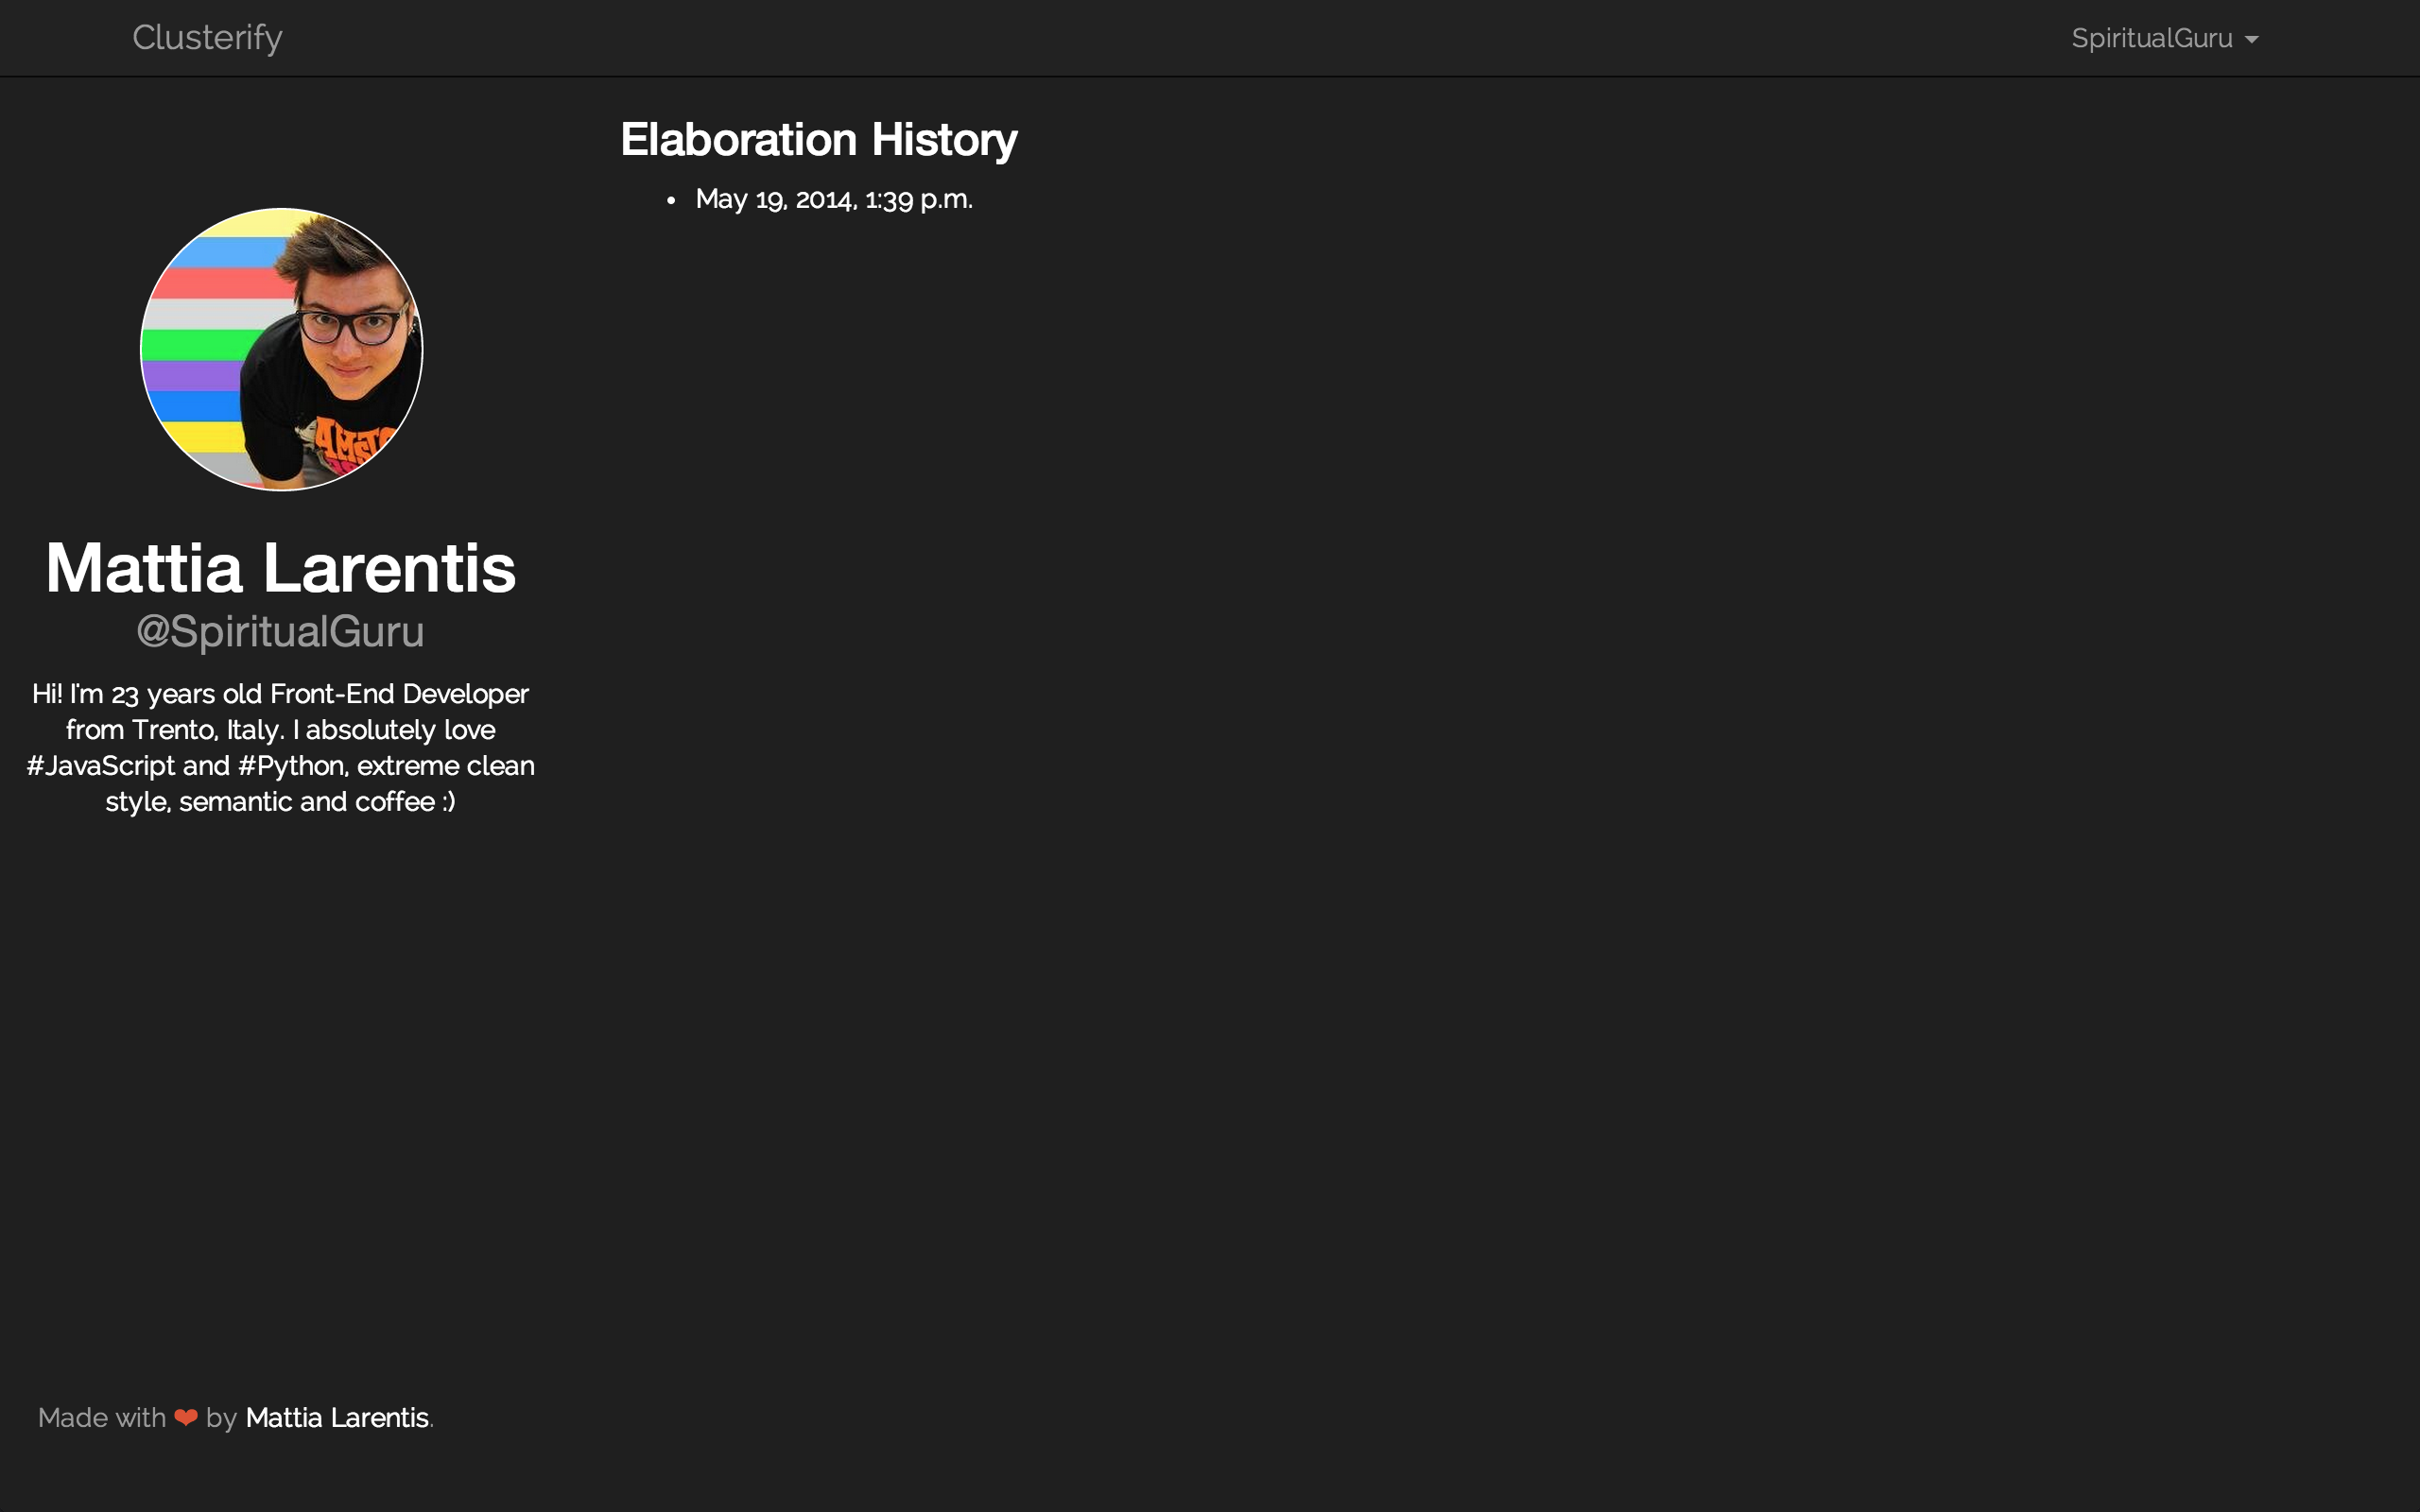
\includegraphics[width=\textwidth]{img/clusterify/history.png}
        	\end{figure}            
	
	\newpage
	Successivamente, si è proposta la questa soluzione a 10 utenti, gli stessi che hanno valutato l'algoritmo di clustering, per capire se fossero sorti altri problemi nell'implementazione della piattaforma. 

	Tutti gli utenti sono rimasti soddisfatti ed il 60\% ha detto che lo userebbe nella vita reale.

